\section{Introduction}

The standard model for cosmology, $\Lambda$CDM cosmology postulates that the Universe is homogeneous, isotropic and contains both cold dark matter (CDM) and dark energy ($\Lambda$). $\Lambda$CDM is very successful at describing the Universe. However there remain many outstanding problems in the model that beg for a solution. One such problem is the mysterious origin of the large-scale magnetic fields permeating the cosmos. Detections of Faraday rotation, synchrotron emissions and Zeeman splitting in distant galaxies and throughout intracluster media reveal weak magnetic fields, on the order of microgauss coherent over the scale of megaparsecs. Though it is easy to amplify existing magnetic fields, for instance with magnetohydrodynamics and galactic dynamos, there is no clear method for producing a seed magnetic field from zero initial conditions.

Primordial magnetic fields (PMFs) are conjectured as seed magnetic fields produced in the early Universe. These weak seed fields - of order nanoguass -  may be produced sometime before recombination and could be taken up by galactic dynamos to become the weak magnetic fields we see today. So far PMFs remain undetected, but the next generations of Cosmic Microwave Background (CMB) experiments beginning over the next decade offer the chance to indirectly observe their effects. Stage-3 CMB experiments such as SPT-3G, Advanced ACTPol and the Simons array will come online in 2016 and 2017. The specifications of the stage-3 experiments are already decided but stage-4 experiments have yet to be designed. It is therefore important to know how sensitive stage-3 experiments will be to the faint traces of PMFs as well as how to best design a stage-4 experiment such that we have the best chance of detecting them. The aim of this thesis is to forecast the upper-limits on PMF detections for stage-3 and stage-4-like CMB experiments.

In this chapter I will begin by discussing the observational evidence of large scale magnetic fields in galaxies and galaxy clusters. In section 1.2 I will give a quick review on CMB observables, polarisation and power spectra - which are instrumental in the study of PMFs. Finally in section 1.3 I will discuss the basic experimental design of stage-3 CMB experiments as well as preliminary figures on stage-4 experiments.

\subsection{Observational Evidence for Large Scale Magnetic Fields}

Galaxy clusters are the largest gravitationally bound objects in the Universe. Each contains thousands of galaxies. Weak microgauss magnetic fields, coherent over mega parsec scales have been observed permeating these clusters and their resident galaxies. Observational evidence of these magnetic fields come in the form of Zeeman splitting, synchrotron emission and Faraday rotation.

\subsubsection{Zeeman Splitting}

In the presence of magnetic fields, electron energy levels in molecules and atoms split based on the angular momentum of the electron with respect to the orientation of the magnetic field, this effect is known as Zeeman splitting. Zeeman splitting can be detected in spectral lines, allowing us to probe magnetic fields in distant sources. Splitting of the Hydrogen 21cm line and the OH 18cm line are common probes of magnetic fields in our own galaxy. Looking further out, Zeeman splitting has also been used to measure the magnetic fields within dense gas clouds around nearby galaxies, with strengths in the order of 0.5-18mG \cite{Robishaw:2008ti}, however these regions are not representative of the large-scale magnetic fields threading the cosmos which are of order microgauss, as measured through synchrotron emissions and Faraday rotation. For the time being Zeeman splitting reaches its limits beyond the neighbouring galaxies, with no constraints on the magnetic fields threading the intracluster medium.

\subsubsection{Synchrotron Emissions}

As electrons and ions spiral around magnetic fields in galaxies and the intracluster medium they emit synchrotron radiation with energies proportional to the strength of the magnetic field and the velocity of the ions \cite{Giovannini:2003yn}.

The emissivity of synchrotron radiation is given by:
\begin{equation}
\label{eqn:synchrotron}
j(B_{\bot},\nu) \propto n_0 B_{\bot}^{(1+\alpha)/2} \nu ^{(1-\alpha)/2}
\end{equation}
where $\nu$ is the frequency of the electron's circular motion, $B_{\bot}$ is the magnetic field component perpendicular to the line of sight and $n_0$ is the normalised electron density, given by $n_e dE = n_0 E^{-\alpha} dE$ where E is the energy of the electron and $\alpha$ is the spectral index, the value for which varies from galaxy to galaxy. \cite{1991A&A...241...47B} measured synchrotron emissions to calculate the magnetic field strength of nearby galaxies and found the average magnetic field strength to be $9 \pm 3 \mu G$ \cite{1991A&A...241...47B}.

\subsubsection{Faraday Rotation}

As photons travel through a magnetised plasma they undergo Faraday Rotation. Magnetised plasmas such as the intracluster medium exhibit different refractive indices for left and right circularly polarised light. Hence, as linearly polarised light propagates through the plasma, its plane of polarisation is rotated by some some angle, $\psi$, given by:

\begin{equation}
\label{eqn:beta}
\psi = RM\lambda^2
\end{equation}

where $\lambda$ is the wavelength of the photon and $RM$ is the rotation measure, given by:

\begin{equation}
\label{eqn:RM}
RM = \frac{e^3}{2\pi ^2 \epsilon_0 m^2 c^3}\int_{0}^{d} n_e(s) B_{\|}(s) ds
\end{equation}

where the prefactors are: $e$, the electron charge, $\epsilon_0$, the vacuum permittivity, $m$, the mass of the electron and $c$, the speed of light in a vacuum. By (2) and (3) the angle of rotation depends on the electron density, $n_e$ in the plasma, the component of the magnetic field parallel to the direction of propagation of the photon, $B_{\|}$ and the photon's wavelength, $\lambda$.

Measurements of Faraday rotation within galaxy clusters have found the magnetic field strength to lie in the range of 0.2 - 3 $\mu G$ \cite{Widrow:2002ud}. In additon, Faraday rotation measurements yield typical magnetic field strengths in galaxies at the level of 4 - 6 $\mu G$ for spiral galaxies and 6 - 8 $\mu G$ in elliptical and irregular galaxies \cite{Widrow:2002ud}.

\subsection{Cosmic Microwave Background Polarisation}
In the last few years CMB polarisation has proven a powerful tool for studying large scale strucutre and the early Universe. If PMFs did in fact exist, then their traces ought to be found within the CMB polarisation. Section 2 contains a discussion on how PMFs affect CMB polarisation.

The CMB is the light from the Big Bang, however the CMB itself didn't form until 300,000 years after the Big Bang. At this point in time the Universe was cool enough to allow photons to decouple from baryons. This event is known as last scattering. From there on the photons were able to free stream through the cosmos. Over the intervening 13 billion years the CMB photons have been cosmologically redshifted into the microwave frequency band. The CMB is a blackbody spectrum corresponding to a temperature of ~2.73K.

\begin{figure}[h]
\centering
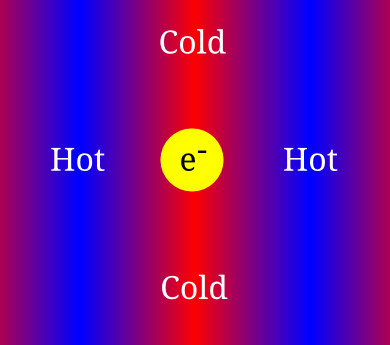
\includegraphics[scale=0.5]{images/quadrupole.png}
\caption{Depiction of a quadrupolar temperature anisotropy that gives rise to CMB polarisation around an electron at recombination. The red regions are the cooler regions, where cool photons approach the electron from and the blue regions are the hotter regions where hotter electrons approach from.}
\label{fig:quadrupole}
\end{figure}

At the time of last scattering the Universe was composed of a hot, ionised plasma, consisting of protons and electrons. The temperature anisotropies in this plasma gave rise to the net polarisation of the CMB that we see today \cite{Hu:1997hv}.
Electrons in the plasma are surrounded by hot and cold patches. Those that are surrounded by quadrupolar temperature anisotropies - two hotter patches either side and then two cooler patches either side on an axis perpendicular to the hotter patches produce a net polarisation through Thomson scattering as shown in figure ~\ref{fig:quadrupole}.

Figure~\ref{fig:thomson} shows how a net linear polarisation arises from Thomson scattering about a quadrupolar temperature anisotropy. Two photons approach the electron from perpendicular directions, one from the cool patch (shown in red) and one from the hot patch (shown in blue). The two photons scatter off the electron perpendicular to the plane of incidence for both photons. The resultant photon has a net linear polarisation oriented in the plane of incidence with an angle of polarisation proportional to the difference in temperature of the two photons. 

\begin{figure}[h]
\centering
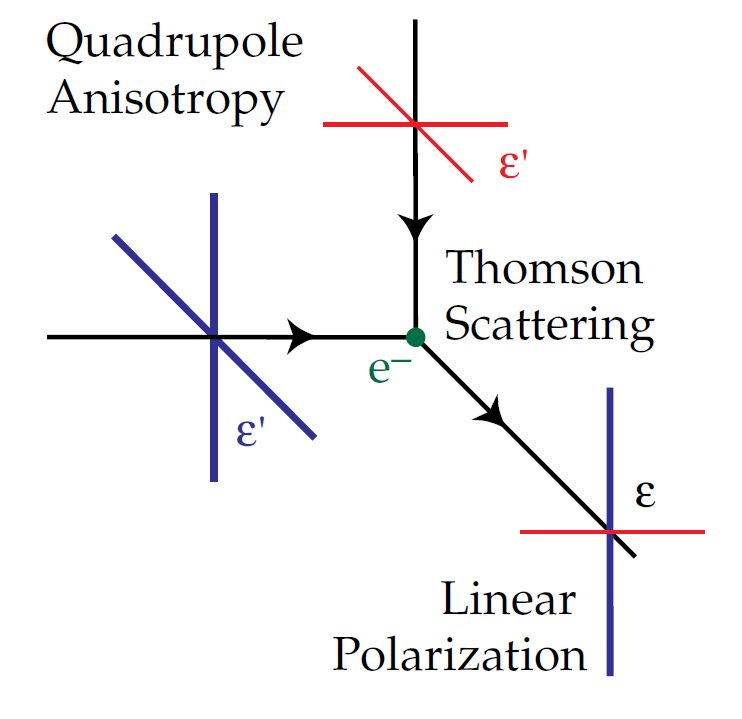
\includegraphics[scale=0.35]{images/thomson.png}
\caption{Thomson scattering of CMB photons in the presence of a quadrupole anisotropy. The red lines are the polarisations of a cold photon and the blue lines are the polarisations of a hot photon both incident on the same electron. The result is a net linear polarisation. Figure from \cite{Hu:1997hv}}
\label{fig:thomson}
\end{figure}

Quadrupolar anisotropies are caused by scalar, vector or tensor perturbations. Scalar perturbations are density fluctuations. Vector perturbations result from vortices in the photon-electron fluid or from more exotic phenomena, such as cosmic strings and other topologcal defects. Finally a tensor perturbation would be the result of gravity waves produced during cosmic inflation.  

In order to describe the effects of perturbations on CMB polarisation we introduce two polarisation modes. E-modes and B-modes. E-modes are formed from scalar perturbations. The E-modes resemble electric fields in electromagnetism in the sense that they are curl-free. The left panel in figure ~\ref{fig:modes} shows the two forms of E-modes. The bottom mode has zero divergence whereas the top mode has non-zero divergence. It is clear to see that E-modes are symmetric under reflection, in other words they have even parity. B-modes on the other hand are formed from vector and tensor perturbations. As we will see in section, B-mode polarisation holds the key to indirectly detecting and constraining the magnitude of PMFs. Continuing the electromagnetism analogy a B-mode resembles a magnetic field, in the sense that it is purely a curl field. Figure ~\ref{fig:modes} shows B-modes on the right panel. There are two forms, each rotating in opposite directions. B-modes are anti-symmetric under reflection - that is reflecting one gives you the other. This property illustrates their characteristic odd parity.

\begin{figure}[h]
\centering
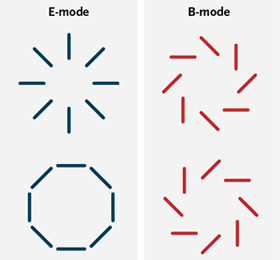
\includegraphics[scale=3]{modes.png}
\caption{Representation of E-mode polarisations and B-mode polarisations. Note how E-modes are symmetric and resemble a divergent field. In contrast the B-modes appear anti-symmetric and resemble a curled field. Figure from \cite{39087c288ce54d4bb9580169e1666880}}
\label{fig:modes}
\end{figure}

\subsection{Future CMB experiments}
This year stage-3 CMB experiments will commence operation and before the end of the next decade, stage-4 CMB experiments will have also collected their data. The next generation of CMB experiments aim to obtain tighter constraints on cosmological parameters such as the tensor-to-scalar ratio as well as map the CMB in higher detail than ever before. Though PMF detection is not the main science goal of these experiments, they will be able to tighten constraints on the primordial magnetic field strength and perhaps make a detection.

Since CMB polarisation has such a faint signal, it is essential that all CMB experiments aim to reduce their level of noise as much as possible. There are many ways to do this - making better detectors or perhaps adding more. In the case of CMB experiments one can produce better detectors by reducing the temperature of the detector. This however has diminishing returns at low temperatures since firstly, lower temperatures are progressively harder to reach and sustain the lower they are. Secondly, current CMB detectors are already well below the temperature of the incoming CMB photons, so the improvement from reducing the temperature any further is negligible.

Instead, the standard approach to lowering noise is to simply add more detectors. This works since photon detection is a Poisson process, that is only discrete numbers of photons can be detected, the rate at which they hit the detector is constant and independent of previous photon detection events and a detector can only detect a single photon at a time. For a Poisson process, the noise level scales with the number of the detectors like: 
\begin{equation}
\label{eqn:noisescaling}
Noise \propto \frac{1}{\sqrt{N_{detectors}}}
\end{equation}
so far, each stage of CMB experiments have added a factor of 10 more detectors, bringing the noise level down by a factor of $\sqrt{10}$.

\begin{table}[b]
\centering
\caption{Properties of Present and Future CMB experiments}
\label{table:future cmb}
\begin{tabular}{l|l|l|l|l}
Experiment & \multicolumn{1}{c|}{Stage} & \multicolumn{1}{c|}{N_{bolo}} & Survey Area ($deg^{2}$)& Polarisation Noise ($\mu$K) \\ \hline
SPT-pol & \multicolumn{1}{c|}{2} & \multicolumn{1}{c|}{1 536} & \multicolumn{1}{c|}{100} & \multicolumn{1}{c}{20} \\
Planck & \multicolumn{1}{c|}{Space-based} & \multicolumn{1}{c|}{-} & \multicolumn{1}{c|}{41 253} & \multicolumn{1}{c}{52} \\
Adv-ACTpol & \multicolumn{1}{c|}{3} & \multicolumn{1}{c|}{2 718} & \multicolumn{1}{c|}{20 000} & \multicolumn{1}{c}{9.9} \\
SPT-3G & \multicolumn{1}{c|}{3} & \multicolumn{1}{c|}{15 234} & \multicolumn{1}{c|}{2 500} & \multicolumn{1}{c}{4.8} \\
Simons Array & \multicolumn{1}{c|}{3} & \multicolumn{1}{c|}{22 764} & \multicolumn{1}{c|}{33 000} & \multicolumn{1}{c}{4.8} \\ 
Stage 4 Expected & \multicolumn{1}{c|}{4} & \multicolumn{1}{c|}{500 000} & \multicolumn{1}{c|}{20 000} & \multicolumn{1}{c}{1.4} \\
\end{tabular}
\\
\begin{flushleft}
This table shows a short (and by no means comprehensive) list of current and upcoming CMB experiments and their key design features useful for detecting PMFs. \cite{Henderson:2015nzj} \cite{Benson:2014qhw} \cite{Suzuki:2015zzg} \cite{Adam:2015vua}. The Planck telescope is the only space-based experiment listed on this table. I have included it because I will use its data release in my analysis. The number of detectors has been left out since the number of detectors on ground and space-based experiment can't be directly compared. For reference Planck has 32 polarisation detectors on its High Frequency Instrument (HFI) and carries out full-sky observations \cite{Lamarre:2003zh}.
\end{flushleft} 
\end{table}

\begin{figure}[h]
\centering
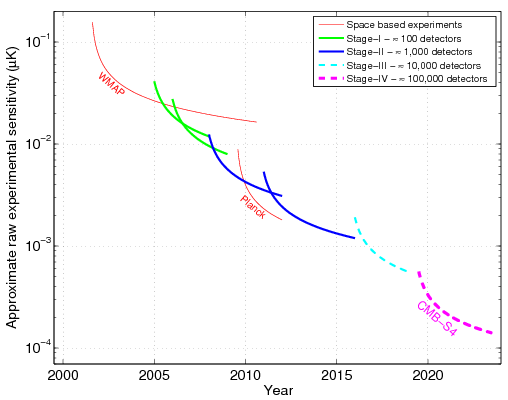
\includegraphics[scale=0.75]{images/experiments.png} 
\caption{Plot of approximate raw experimental sensitivity of CMB experiments vs time in years. The Red lines indicate space-based experiments. Of note is Planck whose sensitivity falls in the middle-range of the stage-2 CMB experiments. The dotted cyan line represents the sensitivity of CMB-S3, which we expect to improve by up to an order of magnitude over Stage 2. CMB-S4 is represented by the dotted purple line, which is set to improve by a further order of magnitude over S3. Figure from \cite{Abazajian:2013oma}}
\end{figure}
